% Options for packages loaded elsewhere
\PassOptionsToPackage{unicode}{hyperref}
\PassOptionsToPackage{hyphens}{url}
\PassOptionsToPackage{dvipsnames,svgnames,x11names}{xcolor}
%
\documentclass[
  singlecolumn,
  9pt]{article}

\usepackage{amsmath,amssymb}
\usepackage{iftex}
\ifPDFTeX
  \usepackage[T1]{fontenc}
  \usepackage[utf8]{inputenc}
  \usepackage{textcomp} % provide euro and other symbols
\else % if luatex or xetex
  \usepackage{unicode-math}
  \defaultfontfeatures{Scale=MatchLowercase}
  \defaultfontfeatures[\rmfamily]{Ligatures=TeX,Scale=1}
\fi
\usepackage[]{libertinus}
\ifPDFTeX\else  
    % xetex/luatex font selection
\fi
% Use upquote if available, for straight quotes in verbatim environments
\IfFileExists{upquote.sty}{\usepackage{upquote}}{}
\IfFileExists{microtype.sty}{% use microtype if available
  \usepackage[]{microtype}
  \UseMicrotypeSet[protrusion]{basicmath} % disable protrusion for tt fonts
}{}
\makeatletter
\@ifundefined{KOMAClassName}{% if non-KOMA class
  \IfFileExists{parskip.sty}{%
    \usepackage{parskip}
  }{% else
    \setlength{\parindent}{0pt}
    \setlength{\parskip}{6pt plus 2pt minus 1pt}}
}{% if KOMA class
  \KOMAoptions{parskip=half}}
\makeatother
\usepackage{xcolor}
\usepackage[top=30mm,bottom=30mm,left=20mm,heightrounded]{geometry}
\setlength{\emergencystretch}{3em} % prevent overfull lines
\setcounter{secnumdepth}{-\maxdimen} % remove section numbering
% Make \paragraph and \subparagraph free-standing
\ifx\paragraph\undefined\else
  \let\oldparagraph\paragraph
  \renewcommand{\paragraph}[1]{\oldparagraph{#1}\mbox{}}
\fi
\ifx\subparagraph\undefined\else
  \let\oldsubparagraph\subparagraph
  \renewcommand{\subparagraph}[1]{\oldsubparagraph{#1}\mbox{}}
\fi


\providecommand{\tightlist}{%
  \setlength{\itemsep}{0pt}\setlength{\parskip}{0pt}}\usepackage{longtable,booktabs,array}
\usepackage{calc} % for calculating minipage widths
% Correct order of tables after \paragraph or \subparagraph
\usepackage{etoolbox}
\makeatletter
\patchcmd\longtable{\par}{\if@noskipsec\mbox{}\fi\par}{}{}
\makeatother
% Allow footnotes in longtable head/foot
\IfFileExists{footnotehyper.sty}{\usepackage{footnotehyper}}{\usepackage{footnote}}
\makesavenoteenv{longtable}
\usepackage{graphicx}
\makeatletter
\def\maxwidth{\ifdim\Gin@nat@width>\linewidth\linewidth\else\Gin@nat@width\fi}
\def\maxheight{\ifdim\Gin@nat@height>\textheight\textheight\else\Gin@nat@height\fi}
\makeatother
% Scale images if necessary, so that they will not overflow the page
% margins by default, and it is still possible to overwrite the defaults
% using explicit options in \includegraphics[width, height, ...]{}
\setkeys{Gin}{width=\maxwidth,height=\maxheight,keepaspectratio}
% Set default figure placement to htbp
\makeatletter
\def\fps@figure{htbp}
\makeatother
% definitions for citeproc citations
\NewDocumentCommand\citeproctext{}{}
\NewDocumentCommand\citeproc{mm}{%
  \begingroup\def\citeproctext{#2}\cite{#1}\endgroup}
% avoid brackets around text for \cite:
\makeatletter
 \def\@biblabel#1{}
 \def\@cite#1#2{{#1\if@tempswa , #2\fi}}
\makeatother
\newlength{\cslhangindent}
\setlength{\cslhangindent}{1.5em}
\newlength{\csllabelwidth}
\setlength{\csllabelwidth}{3em}
\newlength{\cslentryspacing}
\setlength{\cslentryspacing}{0em}
\usepackage{enumitem}
\newlist{CSLReferences}{itemize}{1}
\setlist[CSLReferences]{label={},
  leftmargin=\cslhangindent,
  itemindent=-1\cslhangindent,
  parsep=\parskip,
  itemsep=\cslentryspacing}
\usepackage{calc}
\newcommand{\CSLBlock}[1]{#1\hfill\break}
\newcommand{\CSLLeftMargin}[1]{\parbox[t]{\csllabelwidth}{#1}}
\newcommand{\CSLRightInline}[1]{\parbox[t]{\linewidth - \csllabelwidth}{#1}\break}
\newcommand{\CSLIndent}[1]{\hspace{\cslhangindent}#1}

\usepackage{cancel}
\usepackage{xcolor}
\usepackage[noblocks]{authblk}
\renewcommand*{\Authsep}{, }
\renewcommand*{\Authand}{, }
\renewcommand*{\Authands}{, }
\renewcommand\Affilfont{\small}
\usepackage{cancel}
\makeatletter
\makeatother
\makeatletter
\makeatother
\makeatletter
\@ifpackageloaded{caption}{}{\usepackage{caption}}
\AtBeginDocument{%
\ifdefined\contentsname
  \renewcommand*\contentsname{Table of contents}
\else
  \newcommand\contentsname{Table of contents}
\fi
\ifdefined\listfigurename
  \renewcommand*\listfigurename{List of Figures}
\else
  \newcommand\listfigurename{List of Figures}
\fi
\ifdefined\listtablename
  \renewcommand*\listtablename{List of Tables}
\else
  \newcommand\listtablename{List of Tables}
\fi
\ifdefined\figurename
  \renewcommand*\figurename{Figure}
\else
  \newcommand\figurename{Figure}
\fi
\ifdefined\tablename
  \renewcommand*\tablename{Table}
\else
  \newcommand\tablename{Table}
\fi
}
\@ifpackageloaded{float}{}{\usepackage{float}}
\floatstyle{ruled}
\@ifundefined{c@chapter}{\newfloat{codelisting}{h}{lop}}{\newfloat{codelisting}{h}{lop}[chapter]}
\floatname{codelisting}{Listing}
\newcommand*\listoflistings{\listof{codelisting}{List of Listings}}
\makeatother
\makeatletter
\@ifpackageloaded{caption}{}{\usepackage{caption}}
\@ifpackageloaded{subcaption}{}{\usepackage{subcaption}}
\makeatother
\makeatletter
\makeatother
\ifLuaTeX
  \usepackage{selnolig}  % disable illegal ligatures
\fi
\IfFileExists{bookmark.sty}{\usepackage{bookmark}}{\usepackage{hyperref}}
\IfFileExists{xurl.sty}{\usepackage{xurl}}{} % add URL line breaks if available
\urlstyle{same} % disable monospaced font for URLs
\hypersetup{
  pdftitle={On The Three Wave Panel Design for Causal Inferencee},
  pdfauthor={Joseph A. Bulbulia},
  pdfkeywords={DAGS (Directed Acyclic Graphs), Causal
Inference, Confounding, History, Psychology, Panel},
  colorlinks=true,
  linkcolor={blue},
  filecolor={Maroon},
  citecolor={Blue},
  urlcolor={Blue},
  pdfcreator={LaTeX via pandoc}}

\title{On The Three Wave Panel Design for Causal Inferencee}


  \author{Joseph A. Bulbulia}
            \affil{%
                  Victoria University of Wellington, New Zealand, School
                  of Psychology, Centre for Applied Cross-Cultural
                  Research
              }
      
\date{2023-11-30}
\begin{document}
\maketitle
\begin{abstract}
This article causal diagrams to guide data collection in a three wave
panel design
\end{abstract}
\subsection{Introduction}\label{introduction}

This article explores the benefits of collecting repeated measures data
over at least three waves for causal inference. The advantages of this
approach are made clear through the lens of chronologically ordered
causal diagrams (CITE).

\subsubsection{Step 1. Ask a Causal
Question}\label{step-1.-ask-a-causal-question}

To answer a causal question we must first ask it
(\citeproc{ref-hernuxe1n2016}{Hernán \emph{et al.} 2016}). This question
must clearly specify the exposure (cause) and the outcome (effect), as
well as their temporal relationship, within a defined context.

Suppose we are interested in the effect of religious service attendance
on charitable giving, the causal question should be structured to
clearly delineate these elements.

For example, the question could be framed as: ``Does increasing
attendance at religious services from infrequent (less than once a
month) to frequent (weekly or more) lead to a rise in charitable giving
over a one-year period?'' This question distinctly identifies the nature
of the exposure (increase in frequency of attending religious services)
and the outcome (rise in charitable giving), along with a specific time
frame (one year).

In a three-wave panel design, the timing of the measurements becomes
integral to the study (see: (\citeproc{ref-vanderweele2020}{VanderWeele
\emph{et al.} 2020})). The question must ensure that the temporal order
aligns with the objective of inferring causality. In our case, this
could translate to: ``How does a change in religious service attendance,
measured from the beginning of the year (baseline) to mid-year (wave 1),
influence the levels of charitable giving at the end of the year (wave
2)?'' Here, the change in religious service attendance is captured
between the first and second waves, while the outcome, charitable
giving, is measured in the third wave, establishing a chronological
sequence that tracks the sequence of cause and effect. Ensuring such
temporal ordering is essential to every causal analysis.

Formulating the causal question with such precision is imperative, and
must guide the entire study design, including which variables to measure
and when. It ensures that the study is tailored to address the specific
causal relationship of interest, laying a robust foundation for the
subsequent steps in the causal inference process.

\subsubsection{Step 2. Ensure that the Exposure is Measured at Wave 0
(Baseline) and Wave 1 (An Interval Following
Baseline)}\label{step-2.-ensure-that-the-exposure-is-measured-at-wave-0-baseline-and-wave-1-an-interval-following-baseline}

Measuring the exposure at both baseline (wave 0) and a subsequent
timepoint (wave 1) is crucial in causal inference studies. This approach
provides several key benefits:

\begin{enumerate}
\def\labelenumi{\arabic{enumi}.}
\item
  \textbf{Incidence Effect Interpretation}: By including baseline data,
  we can distinguish between incidence (new occurrences) and prevalence
  (existing states) effects. For instance, in a study on religious
  service attendance, this approach allows us to differentiate the
  effect of starting to attend services regularly from the effect of
  ongoing attendance.
\item
  \textbf{Confounding Control}: Measuring exposure at baseline helps
  control for time-invariant confounders. These are factors that do not
  change over time and might affect both the exposure and the outcome.
  In the context of religious service attendance, personal attributes
  like inherent religiosity could influence both attendance and related
  outcomes.
\item
  \textbf{Sample Adequacy Evaluation}: For rare exposures, baseline
  measurements can assess sample size adequacy. If a change in exposure
  is infrequent (e.g., infrequent to weekly religious service
  attendance), a larger sample may be needed to detect causal effects.
  By measuring exposure at baseline, researchers can better evaluate
  whether their sample is representative and large enough to detect such
  rare changes.
\end{enumerate}

\subsubsection{Step 3. Ensure that the Outcome is Measured at Wave 0
(Baseline) and Wave 2 (An Interval Following Wave
1)}\label{step-3.-ensure-that-the-outcome-is-measured-at-wave-0-baseline-and-wave-2-an-interval-following-wave-1}

Measuring the outcome at both baseline (wave 0) and after the exposure
(wave 2) is essential for several reasons:

\begin{enumerate}
\def\labelenumi{\arabic{enumi}.}
\item
  \textbf{Temporal Ordering}: Measuring the outcome at baseline and then
  again after the exposure (wave 2) ensures the correct temporal
  sequence. This approach helps to establish that the exposure precedes
  the outcome, which is fundamental in establishing a causal
  relationship.
\item
  \textbf{Confounding Control}: Including the baseline measure of both
  the exposure and outcome allows for better control of confounding.
  This approach helps to isolate the effect of the exposure on the
  outcome from wave 1 to wave 2, independent of their baseline levels.
  It reduces the risk of confounding, where unmeasured factors might
  influence both the exposure and the outcome.
\item
  \textbf{Robustness Checks}: Baseline outcome measurements provide a
  basis for conducting robustness checks and sensitivity analyses. These
  checks are essential for detecting outliers, errors in data
  collection, and understanding the stability of the measured phenomena
  over time.
\end{enumerate}

\begin{figure}

{\centering 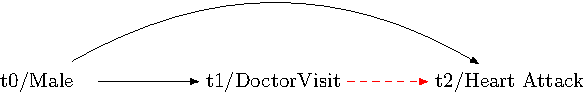
\includegraphics[width=0.8\textwidth,height=\textheight]{notes-three-wave-panel_files/figure-pdf/fig-dag-1-1.pdf}

}

\caption{\label{fig-dag-1}Causal diagram adapted from Vanderweele et
al.'s three-wave panel design (VanderWeele et al.~2020). The dotted line
indicates a reduction in bias arising from including baseline measures
for the exposure and outcome. For an unmeasured confounder U to bias the
exposure-outcome association, it would need to do so independently of
these outcome and exposure baseline measures. The graph clarifies that
by measuring confounders before the exposure and the exposure before the
outcome, we reduce the potential for reverse causation, collider
stratification, and mediator biases.}

\end{figure}

\subsubsection{Step 4. Identify Observable Common Causes of the Exposure
and the
Outcome}\label{step-4.-identify-observable-common-causes-of-the-exposure-and-the-outcome}

Next, we must identify and record at wave 0 (baseline) all potential
confounders that could influence both the exposure (e.g., frequency of
attending religious services) and the outcome (e.g., charitable giving).
Proper identification and adjustment for these confounders are crucial
for accurate causal inference.

\begin{enumerate}
\def\labelenumi{\arabic{enumi}.}
\item
  \textbf{Defining Confounders}: Confounders are variables that are
  associated with either the exposure or the outcome, or that might be a
  descendent of a common cause of both. We should exclude from this set
  any variable that is an instrumental variable. For example, in the
  context of religious service attendance and charitable giving,
  socioeconomic status (SES) could be a confounder. Individuals with
  higher SES might be more likely to attend religious services regularly
  and also have greater financial capacity for charitable giving. We
  should ensure that good measures of SES are obtained at baseline.
\item
  \textbf{Measurement of Confounders}: Confounders should be measured at
  baseline (wave 0) to ensure that their relationship with both the
  exposure and outcome is properly understood and accounted for. This
  measurement helps in disentangling the true effect of the exposure on
  the outcome from the effects of these confounding variables.
\item
  \textbf{Grouping Confounders for Efficiency}: To maintain clarity in
  analysis, it is advisable to group confounders under standard labels
  when they have similar functional roles in the causal diagram. For
  instance, demographic factors like age, gender, and education level
  can be grouped together if they serve similar roles in influencing
  both religious service attendance and charitable giving.
\item
  \textbf{Use Causal Diagrams}: Causal diagrams allow us to visualise
  causal relationships among variables.
\item
  \textbf{Minimize Mediation Bias}: Recording confounders before the
  exposure occurs is critical for minimizing mediation bias. Mediation
  bias can arise when a variable is both a confounder and a mediator in
  the causal pathway. By identifying and adjusting for these variables
  at baseline, we can reduce the risk of incorrectly attributing the
  effect of the exposure to a mediator.
\end{enumerate}

\subsubsection{Step 5. Gather data for proxy variables of unmeasured
common causes at the baseline
wave}\label{step-5.-gather-data-for-proxy-variables-of-unmeasured-common-causes-at-the-baseline-wave}

If any unmeasured confounders influence both the exposure and outcome,
but we lack direct measurements, we should make efforts to include
proxies for them. Even if this strategy cannot eliminate all bias from
unmeasured confounding, it will generally reduce bias.

\subsubsection{Step 6. State the target population for whom the causal
question
applies}\label{step-6.-state-the-target-population-for-whom-the-causal-question-applies}

We need to define for whom our causal inference applies. For this
purpose, it is helpful to distinguish the concepts of source population
and target population and between the concepts of generalisability and
transportability.

\begin{enumerate}
\def\labelenumi{\arabic{enumi}.}
\item
  \textbf{The source population} is the population from whom our sample
  is drawn.
\item
  \textbf{The target population} is the larger population for whom we
  aim to apply our study's results. The closer the source population
  matches the target population in structural features relevant to our
  causal questions, the stronger our causal inferences about the target
  population will be.
\item
  \textbf{Generalisability}: when the causal effect estimated from a
  sample applies to the target population beyond the sample population,
  we say the causal effect estimates are generalisable. This concept is
  also known as ``external validity.''
\end{enumerate}

Let \(PATE\) denote the population average treatment effect for the
target population. Let \(ATE_{\text{source}}\) denote the average
treatment effect in the source population. Let \(W\) denote a set of
variables upon which the source and target population structurally
differ. We say that results \emph{generalise} if there is a function
such that:

\[PATE =  f(ATE_{\text{source}}, W)\]

\begin{enumerate}
\def\labelenumi{\arabic{enumi}.}
\setcounter{enumi}{3}
\tightlist
\item
  \textbf{Transportability}: when causal effects estimates may
  generalise to different settings and populations from which the source
  population was sampled, we say effects are transportable. Where \(T\)
  denotes a set of variables upon which the source and the target
  population structurally differ, we say that results are transportable
  if there is a function such that
\end{enumerate}

\[ATE_{\text{target}} \approx f(ATE_{\text{source}}, T)\]

This function similarly maps the average treatment effect from the
source population to a target population. The function over \(T\) might
be more complex, as it must handle potential heterogeneity of effects
and unobserved sources of bias. To assess transportability, we generally
require information about the source and target populations and a
specialist understanding.

\subsubsection{Step 7. Retain Sample}\label{step-7.-retain-sample}

Maintaining a stable sample over the course of a three-wave panel study
is critical for ensuring the validity of causal inferences. Panel
attrition, where participants drop out of the study over time, can
introduce significant biases. Therefore, strategies for sample retention
are essential for data collection that is purpose built for causal
inference.

\begin{enumerate}
\def\labelenumi{\arabic{enumi}.}
\item
  \textbf{Developing Tracking Protocols}: Establish robust systems for
  tracking participants over the study period. This involves keeping
  updated records of contact information such as addresses, emails,
  phone numbers, and names, and accounting for changes over time.
  Advanced tracking methods might include periodic contact or follow-ups
  to keep the records current.
\item
  \textbf{Motivational Strategies for Retention}: Implement strategies
  to encourage ongoing participation. This can involve regular
  communication about the study's progress and impact, providing
  incentives for continued participation, or making the process as
  convenient as possible for participants. The key is to engage the
  participants in a way that motivates them to stay involved.
\item
  \textbf{Inclusivity in Participant Engagement}: Ensure that retention
  strategies are inclusive and cater to the diverse needs of the
  population under study. This might involve tailoring communication or
  incentives to different subgroups within the population or addressing
  specific barriers to continued participation that certain groups might
  face.
\item
  \textbf{Use Local Knowledge}: Engage with specialists who have
  in-depth knowledge of the population under study. They can provide
  insights into the most effective strategies for retaining different
  groups within the population.
\item
  \textbf{Participant Feedback and Adaptation}: Incorporate feedback
  from participants to improve retention strategies. This could involve
  regular surveys or feedback sessions to understand participants'
  experiences and adjust the study procedures accordingly.
\item
  \textbf{Addressing Potential Bias from Attrition}: Even with robust
  retention strategies, some degree of attrition is often inevitable.
  Plan for potential attrition from the outset by over-sampling and
  always include methods for adjusting for it at the analysis phase.
\item
  \textbf{Continual Monitoring and Response}: Continuously monitor the
  rate and patterns of attrition throughout the study and implement
  responsive strategies as needed. This could involve targeted
  re-engagement efforts or adjustments in study procedures to address
  emerging challenges.
\item
  \textbf{Documentation and Reporting}: Carefully document all retention
  efforts and the patterns of attrition that occur in the study. This
  documentation is crucial for interpreting the study results and for
  informing future research.
\end{enumerate}

Sample retention is mission-critical for preventing bias arising to
panel attrition in three-wave panel designs. Researchers must be aware
of it, and combat it.

\subsection*{References}\label{references}
\addcontentsline{toc}{subsection}{References}

\phantomsection\label{refs}
\setlength{\cslentryspacing}{0em}
\begin{CSLReferences}
\bibitem[\citeproctext]{ref-hernuxe1n2016}
Hernán, MA, Sauer, BC, Hernández-Díaz, S, Platt, R, and Shrier, I (2016)
Specifying a target trial prevents immortal time bias and other
self-inflicted injuries in observational analyses. \emph{Journal of
Clinical Epidemiology}, \textbf{79}, 7075.

\bibitem[\citeproctext]{ref-vanderweele2020}
VanderWeele, TJ, Mathur, MB, and Chen, Y (2020) Outcome-wide
longitudinal designs for causal inference: A new template for empirical
studies. \emph{Statistical Science}, \textbf{35}(3), 437466.

\end{CSLReferences}



\end{document}
